\documentclass[a4paper,11pt,oneside]{book}

% packages 
\usepackage{arsclassica}    % fancy layout
\usepackage[english]{babel}\addto{\captionsenglish}{\renewcommand{\bibname}{References}}
\usepackage{caption}         % figure captions
\usepackage[square,numbers,super,sort&compress]{natbib}  % bibliography style
\usepackage[cc]{titlepic}    % enable logo on title page
\usepackage{graphicx}       % logo related
\usepackage{multirow}

\usepackage{standalone}
\standalonetrue

% Margins for pretty version ::
%\usepackage[pass]{geometry}
% Margins for university regulations ::
\usepackage[top=2cm, bottom=4cm, left=4cm, right=2.5cm]{geometry}
\usepackage{setspace}
\onehalfspacing

% don't hang captions
\captionsetup{format=plain}

% bibliography
\bibliographystyle{../thesis}

\graphicspath {{../figs/}}

\begin{document}

%\maketitle

\chapter{Local chromatin conformation}\label{chap:shh}

\section{Introduction}

The Hi-C assay provides a genome-wide overview of chromatin conformation, however the broad scope of this all-versus-all assay places inherent limits on the resolution at which individual interactions can be analysed. For a closer look at chromatin conformation within a region of interest, alternative C-based assays such as 3C, 4C and 5C can be employed alongside classical microscopy techniques like FISH.

Here I discuss a collaborative project within the IGMM (with members of Prof. Robert Hill's laboratory) involving the use of 4C and 5C data to zoom in on a particularly well-studied locus involved in limb development: the Sonic hedgehog (\emph{Shh}) gene and its distal \emph{cis}-regulatory element named ZRS.

\section{The SHH locus}

\begin{figure}
\begin{center} 
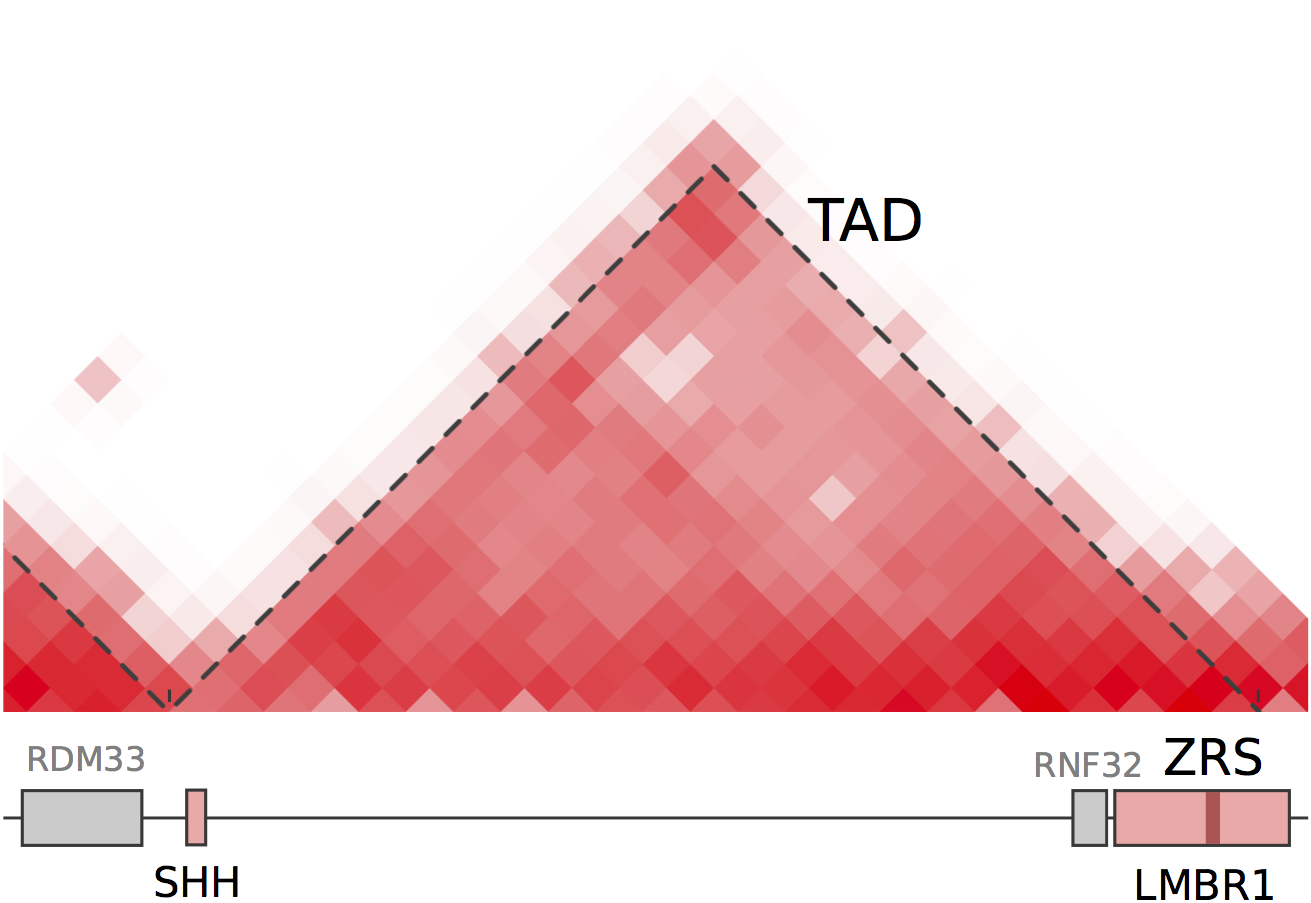
\includegraphics[width=3.5in]{shhtad.png}
\captionsetup{width=\textwidth} 
\caption[ZRS--\emph{Shh} contacts occur within a stable TAD.]{ {\bf ZRS--\emph{Shh} contacts occur within a stable TAD. }
An approximately 1 Mb region of the mouse genome is shown below a matched section of a Hi-C contact map (derived from previously published data\cite{Dixon2012}). A clear TAD can be identified spanning from the \emph{Shh} gene to the ZRS, dashed lines show TAD boundaries called by \citet{Dixon2012} %The heatmap was generated for \citet{Anderson2014a}
}\label{fig:shhtad}
\end{center} 
\end{figure} 

% , and is conserved across mammals and fish

Anterior-posterior patterning in the developing limb is regulated in mammals by the Sonic hedgehog morphogen, encoded by the \emph{Shh} gene.\cite{Anderson2012} Specifically, the \emph{Shh} gene is expressed within a confined region of developing limb buds named the "zone of polarising activity" (ZPA). Its expression within this region is known to be regulated by a well-studied enhancer, the "ZPA regulatory sequence" or ZRS.\cite{Hill2013a} ZRS is located almost 1 Mb downstream of its target \emph{Shh} promoter in humans (nearer 800 kb in mouse), and is located in intronic regions of another gene, LMBR1 (Fig. \ref{fig:shhtad}).\cite{Hill2013a, Laurell2012} Expression of \emph{Shh} within the ZPA is tightly controlled, initiating in mice at developmental stage E$9.5$ and terminating at E$12.5$.\cite{Amano2009} As such, single point mutations and short insertions within the ZRS enhancer have been linked to various limb deformities, including pre- and post-axial polydactyly.\cite{Anderson2012, Lettice2008, Laurell2012} For example, a heritable point mutation in the ZRS enhancer is the cause of polydactyly in "Hemingway cats", a large group of domestic cats with extra toes that reside at the former home of Ernest Hemingway.\cite{Lettice2008, Zeller2009}  

To further investigate the dynamics of the \emph{Shh} locus, our collaborators in the Hill lab (IGMM, University of Edinburgh) have developed a model system which allows inducible \emph{Shh} expression in a non-expressing 14fp cell line derived from the developing murine limb bud. Treatment of this cell line with the histone deacetylase inhibitor trichostatin A (TSA) then leads to detectable \emph{Shh} expression, and increased levels of the histone activation mark H3K27ac at the ZRS (\emph{unpublished data}). However, the question remains whether this TSA treatment is fundamentally altering local chromatin structure---that is, bringing together the ZRS enhancer with its target \emph{Shh} promoter---or whether ZRS and \emph{Shh} are in contact in both the active and non-expressing cell lines in a poised state. Previous 3D-FISH experiments have shown the ZRS--\emph{Shh} contact  to be associated with \emph{Shh} expression in the developing limb bud, though it is not detected in every cell.\cite{Amano2009, Hill2013a} Instead only a proportion of cells in the ZPA are \emph{Shh}-expressing at a given time, and it is thought that the ZRS--\emph{Shh} colocalisation is most likely to occur within these expressing cells.\cite{Amano2009}
%Alternatively, studies have previously reported the \emph{Shh}--ZRS interaction is an example of a "pre-formed loop", and as such is maintained regardless of transcriptional activity.\cite{Bouwman2015a}

My part in this collaboration was to analyse 3C-seq (also known as 4C), then 5C data generated by our collaborators over the \emph{Shh}--ZRS region in mouse. Experimental design and wet-lab procedures were performed by members of the Hill lab.

\section{4C of the ZRS}\label{sec:4cshh}

4C experiments were performed by collaborators using the ZRS region as a bait sequence, or "viewpoint", such that ZRS contacts were measured with all other HindIII restriction fragments genome-wide. Thus the 4C technique allows us to assay changes in the ZRS--\emph{Shh} contact relative to the totality of other chromatin interactions involving ZRS.

The 4C experimental design involved two control experiments. The first used cells derived from whole limb bud at developmental stage E11.5, thereby containing some \emph{Shh} expressing cells as a positive control. The negative control was a mouse mandibular cell line (MD) which does not express \emph{Shh}. Expression status in each case was experimentally verified (\emph{data not shown}). For the perturbation experiment, 4C was performed in the \emph{Shh}-inducible 14fp cell line, both with and without trichostatin A (TSA) treatment.

\subsection{4C pipeline}

The 4C analysis pipeline, starting from de-multiplexed sequencing reads (\texttt{fastq} files) as produced by our in-house sequencing facilities using an Ion Torrent Ion Proton\textsuperscript{TM} sequencer, can be summarised as:

\begin{enumerate}
\item Trim known bait sequence using \texttt{cutadapt},\cite{cutadapt} select only those reads where known viewpoint-associated sequence was present
\item Map reads to the mouse reference genome (build \texttt{mm9}) using \texttt{bowtie2}\cite{Langmead2012} with the \texttt{very-sensitive} flag
\item Filter alignments with a MAPQ score $>30$ to select for high-confidence alignments using \texttt{samtools}\cite{Li2009}
\item Normalise contacts using the \texttt{r3cseq} R package and assign FDR $q$-values to interactions, with the aim of finding those significantly over-represented relative to expectation (Methods \ref{methods:4c})
\end{enumerate}

% Adam sent a powerpoint he gave for section meeting, see also Prof Hill's publications

\subsection{ZRS--\emph{Shh} interaction following TSA treatment}

\begin{figure}
\begin{center} 
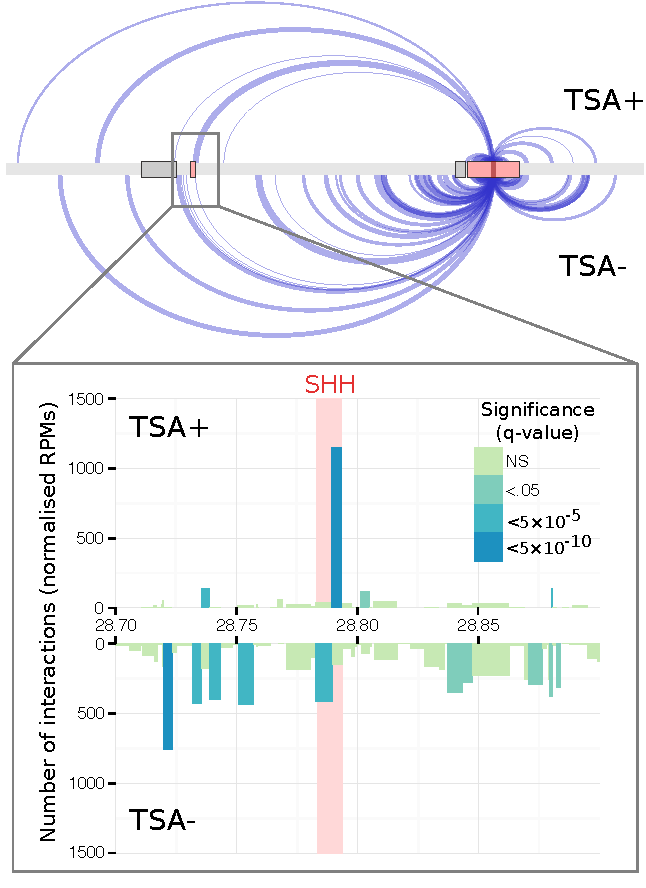
\includegraphics[width=5in]{shharc_full.pdf}
\captionsetup{width=\textwidth} 
\caption[TSA treatment induces a strong ZRS--\emph{Shh} interaction. ]{ {\bf TSA treatment induces a strong ZRS--\emph{Shh} interaction. }
4C interactions are shown as edges from source node (ZRS enhancer bait fragment) to targets along an approximately 2 Mb region of chromosome 5. Edge width is proportional to the number of interactions, only highly significant interactions are shown (FDR $q$-value $<5 \times 10 ^{-5}$; Methods \ref{methods:4csignif}). Zoomed region shows the number of interactions of the bait region with \emph{Shh} in both untreated and TSA treated (after 24h) samples. Each green--blue rectangle is a restriction fragment, coloured by FDR $q$-value indicating the significance of the interaction above expected levels.
}\label{fig:ssharc}
\end{center} 
\end{figure} 


The results of a comparison between 4C experiments in TSA treated and untreated 14fp cells is shown in Figure \ref{fig:ssharc}. In it we see a striking and highly significant ZRS--SHH contact in the treated sample ($q$-value $ < 5 \times 10^{-10}$), with a weaker but still significant contact in the adjacent restriction fragment in the untreated sample ($q$-value $ < 5 \times 10^{-5}$). 

\begin{figure}
\begin{center} 
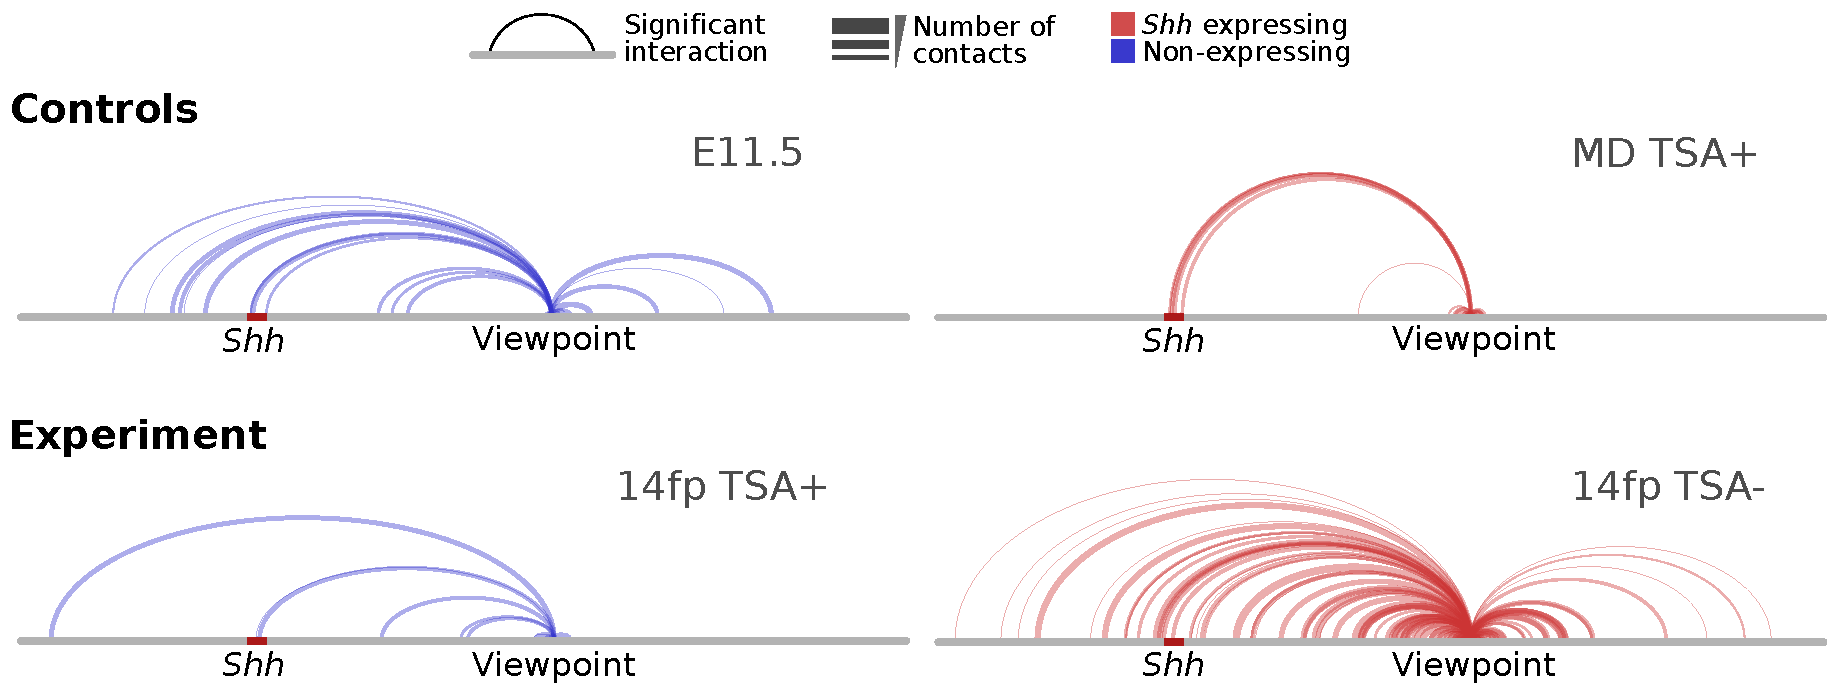
\includegraphics[width=5.5in]{4c_4way.pdf}
\captionsetup{width=\textwidth} 
\caption[ TSA treatment in 14fp cells results in a more specific ZRS--\emph{Shh} contact. ]{ {\bf TSA treatment in 14fp cells results in a more specific ZRS--\emph{Shh} contact. }
Arc plots are shown for two control experiments: the \emph{Shh} expressing E11.5 whole limb bud and non-expressing mandibular cell line (MD). Also shown is the 14fp inducible cell line, with and without treatment with trichostatin A (TSA) after 18 hours. Arcs link significant interactions ($q$-value $< 0.05$) and arc widths are proportional to the normalised number of reads recorded for the interaction (Methods \ref{methods:4c}).
}\label{fig:4c4way}
\end{center} 
\end{figure} 

Comparing these results with controls shows a detectable and significant ZRS--\emph{Shh} contact in each case, regardless of \emph{Shh} expression status (FDR $q$-value $ < 0.05$); Fig. \ref{fig:4c4way}). This is in agreement with previous evidence suggesting ZRS contacts \emph{Shh} constitutively.\cite{Bouwman2015a} However the TSA-- 14fp cell line also shows a large number of off-target contacts, potentially indicating a lack of specificity in the ZRS--\emph{Shh} contact, or a range of alternative contacts occurring throughout the cell population.

Unpublished experimental results show that following TSA treatment, \emph{Shh} expression increases over a period of 24 hours until it reaches that seen in the limb, this steady increase is also mirrored by an increase in the level of H3K27ac histone mark over ZRS (Hill lab, \emph{personal communication}). For this reason, 4C of ZRS was also performed a full 24 hours after TSA treatment, as well as the 18 hour treatment analysed above (e.g. Fig. \ref{fig:4c4way}). These two experiments give largely similar results (Fig. \ref{fig:4carcs}), and the ZRS--\emph{Shh} interaction frequency is highly significant in each case, particularly 24 hours after treatment (\emph{TSA-} : $ q < 1.5 \times 10^{-5}$; \emph{TSA+}$^{18h}$ : $q < 1.4 \times 10^{-8}$; \emph{TSA+}$^{24h}$ : $ q < 7.8 \times 10^{-35}$).

Additional FISH data produced by our collaborators shows approximately equal levels of compaction in this region in both TSA treated and untreated 14fp cells (\emph{data not shown}). This information in combination with the 4C results reported here (Fig. \ref{fig:ssharc}) support a hypothesis that as these two loci border a TAD (Fig. \ref{fig:shhtad}), they frequently contact each other regardless of \emph{Shh} expression state. It could also be the case that TSA treatment brings about a more specific, functional ZRS--\emph{Shh} contact in 14fp cells which is coupled with expression of the \emph{Shh} gene.

\begin{figure}
\begin{center} 
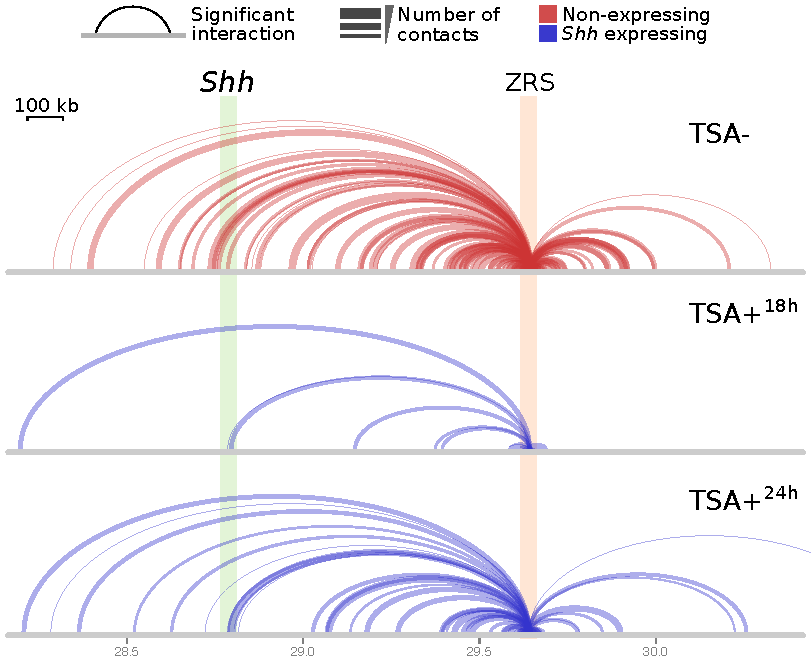
\includegraphics[width=4.6in]{4cArcs_v2.pdf}
\captionsetup{width=\textwidth} 
\caption[ A stable ZRS--\emph{Shh} interaction is coupled with reduced extraneous contacts. ]{ {\bf A stable ZRS--\emph{Shh} interaction is coupled with reduced extraneous contacts. }
Arc plots are shown for an untreated, non-expressing 14fp cell population (\emph{TSA-}) and following TSA treatment after 18 and 24 hours. Arcs link significant interactions ($q$-value $< 0.05$) and arc widths are proportional to the normalised number of reads recorded for the interaction (Methods \ref{methods:4c}).
}\label{fig:4carcs}
\end{center} 
\end{figure} 

\subsection{Assay diagnostics}

The 4C protocol used by our collaborators in this work was that of \citet{Stadhouders2013} In it, the authors advise some statistical tests to ensure the quality of the experiment results. Among these were:\cite{Stadhouders2013}

\begin{enumerate}
\item Sequencing reads should be found to have high duplication rates of $95\%$ or greater.
\item $50\%$ or more of all reads should map to the chromosome on which the bait region is located.
\end{enumerate}

% duplication: treated 02 : 71.2 % (reads 42.2M)
%                                 04 : 84.4 % (reads 24.2M)
%                    haeiii: 74.0% (reads 10.4M)
%                    mluci: 62.8% (reads 10M)

Additionally, the 4C procedure was adapted for specific in-house sequencing instruments (an Ion Torrent Ion Proton\textsuperscript{TM} sequencer as opposed to Illumina\textsuperscript{TM} technology) and as such required diagnostics to confirm the experimental data was accurate. 

Sequence duplication levels were measured with \texttt{FastQC}\cite{fastqc} and are shown in Table \ref{tab:4c}. We find slightly lower than expected levels of duplication, ranging from $62.8\%$ to $84.4\%$. This suggests that while the assay does appear to be working, there may be extraneous noise and non-bait interactions in the sequencing library.

\begin{table}[]
\centering
\caption[4C sequencing library statistics.]{ {\bf 4C sequencing library statistics.}
4C experiments are summarised as total number of reads in each experiment and the percentage of those reads labelled "duplicates". Note in 4C these duplicates are not artifactual and instead result from large numbers of contacts nearby to the viewpoint.
}
\label{tab:4c}
%\begin{tabular}{lcccc} % We use MlucI, don't show HaeIII, confusing
%                                      & \multicolumn{2}{c}{{\bf TSA-}}      & \multicolumn{2}{c}{{\bf TSA+}}   \\ \cline{2-5} 
%\multicolumn{1}{l|}{}                 & MlucI & \multicolumn{1}{c|}{HaeIII} & 18h  & \multicolumn{1}{c|}{24h}  \\ \hline
%\multicolumn{1}{|l|}{Reads (Million)} & 10    & \multicolumn{1}{c|}{10.4}   & 8.8 & \multicolumn{1}{c|}{24.2} \\ \cline{2-5} 
%\multicolumn{1}{|l|}{Duplicated (\%)} & 62.8  & \multicolumn{1}{c|}{74.0}   & 74.2 & \multicolumn{1}{c|}{84.4} \\ \hline
%\end{tabular}
\begin{tabular}{l|c|cc|c|c|}
\cline{2-6}
                                      & \multirow{2}{*}{{\bf 14fp TSA-}} & \multicolumn{2}{c|}{{\bf 14fp TSA+}} & \multirow{2}{*}{{\bf E11.5}} & \multirow{2}{*}{{\bf MD TSA+}} \\
                                      &                                  & 18h               & 24h              &                              &                                \\ \hline
\multicolumn{1}{|l|}{Reads (million)} & 10.0                             & 8.8               & 24.2             & 10.7                         & 12.2                           \\
\multicolumn{1}{|l|}{Duplicated (\%)} & 62.8                             & 74.2              & 84.4             & 80.2                         & 72.8                           \\ \hline
\end{tabular}
\end{table}


Unfortunately we found the proportion of reads mapped to the bait region chromosome, chromosome 5 in this case, fell below the prescribed level of $50\%$. Across 4C experiments, we find instead that between approximately $10$--$20\%$ of all reads mapped to the bait chromosome (Fig. \ref{fig:4cchromosomes}), except for  the 18 hour TSA+ treatment experiment which shows only around $7\%$. While this is still a clear enrichment over non-bait chromosomes, relative to their lengths, it suggests the assay results suffer from either increased \emph{trans}-contact noise or decreased \emph{cis}-contact enrichment around the bait region. 

\begin{figure}
\begin{center} 
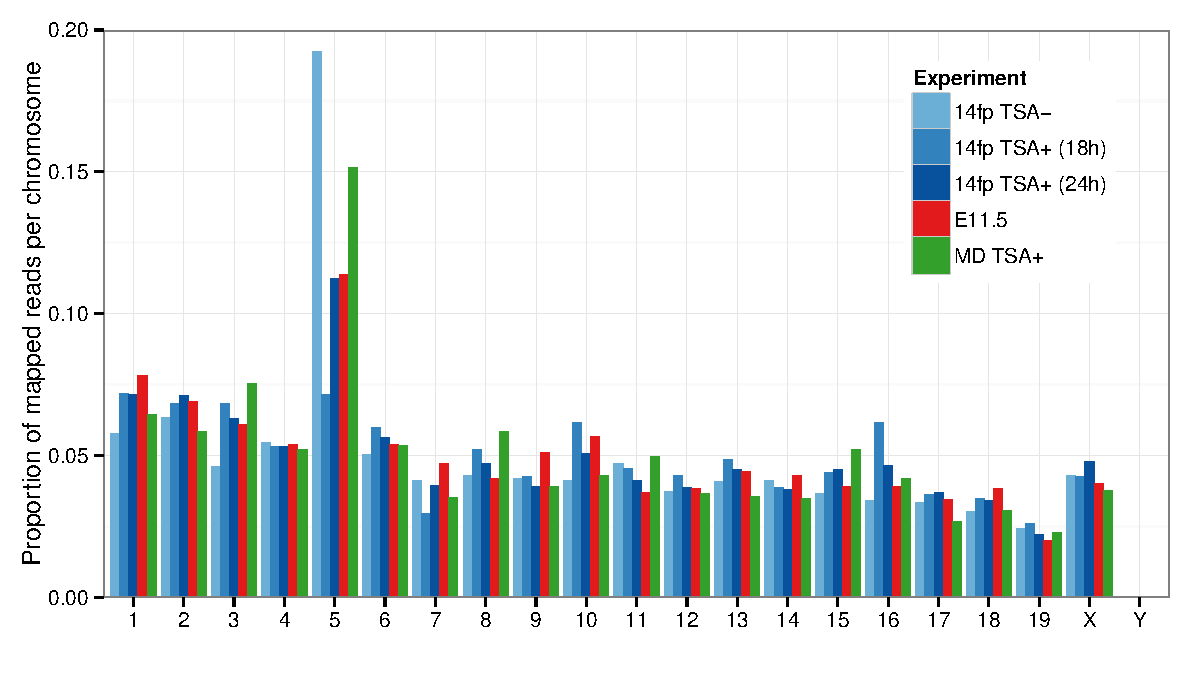
\includegraphics[width=5.4in]{4c_chromosomes_v2.pdf}
\captionsetup{width=\textwidth} 
\caption[ The bait chromosome is enriched for 4C sequencing reads. ]{ {\bf The bait chromosome is enriched for 4C sequencing reads. }
Chromosome 5 is visibly enriched for 4C reads as it  contains the ZRS bait region (or viewpoint). Experiments include treated and untreated 14fp cells (TSA-, TSA+$^{18h}$, TSA+$^{24h}$) as well as positive control (E$11.5$) and negative control (MD TSA+).
}\label{fig:4cchromosomes}
\end{center} 
\end{figure} 

Lower than expected levels of both sequence duplication and bait chromosome enrichment suggest loss of signal around the bait region itself. This is the area where we expect both very high levels of duplication (identical restriction fragment pairings between nearby genomic locations) and where a majority of all sequencing reads should originate, driving the overall chromosome enrichment seen in Figure \ref{fig:4cchromosomes}. The precise reason for the discrepancy is unclear but suggests the results of the assays performed by collaborators may have a lower signal-to-noise ratio than has previously been achievable in 4C experiments.\cite{Stadhouders2013} Potentially the signal-to-noise ratio could be improved by utilising a double cross-linking procedure such as that used in \citet{Lin2012}

\section{Polymer modelling}

% intro stuff introducing 3d modelling
Chromosome conformation capture assays permit the exploration of genome organisation, but such data are commonly analysed using one or two-dimensional representations. A growing set of algorithms looks instead to rebuild the three-dimensional trajectory of a chromatin fibre, using Hi-C or 5C data as input (e.g. \citenum{Bau2011a, Hu2013a, Varoquaux2014a, Lesne2014, Trieu2014, Peng2013, Ay2014b, Caudai2015}). Intuitively, in each method the interaction frequency between two regions is idealised as inversely proportional to their physical distance (and adjusted according to various other constraints). Where these methods differ is in their approaches to performing this spatial transformation, and in solving the subsequent optimisation problem. We chose the \texttt{AutoChrom3D} method\cite{Peng2013} for use in this work (described in Section \ref{sec:achrom}) as the algorithm can accept 5C input and model polymers at high resolutions of up to 8 kb.

\subsection{\texttt{AutoChrom3D} method}\label{sec:achrom}

The procedure implemented in \texttt{AutoChrom3D} can be summarised as:\cite{Peng2013}

\begin{enumerate}
\item The chromatin fibre is represented as beads-on-a-string, with $N_{beads} = \lceil\frac{L}{R}\rceil$ (where $L$ is the length of the region and $R$ the resolution)
\item A local compaction parameter is calculated using a sliding window of each 50 adjacent beads (intra-window contacts are averaged and compared to those over the whole region under study)
\item Interaction frequency between beads of a given genomic distance is modelled as a Poisson-distributed random variable and noisy or unstable contacts, considered in the context of neighbouring beads, are filtered
\item This filtered set of interaction frequencies are then normalised using the previously-calculated compaction parameter to give an $N_{beads} \times N_{beads}$ matrix of interaction strengths
\item Interaction strength is converted to spatial distance through two linear transformations based on experimental observations of nuclear occupancy and regional flexibility\cite{Kalhor2012}
\item Cartesian co-ordinates are then calculated via non-linear constrained optimisation of pairwise spatial distances using LINGO\cite{lingo}
\end{enumerate}

\subsection{Modelling the \emph{Shh} region with 5C}\label{sec:shh5c}

5C data was generated by our collaborators over the same ZRS--\emph{Shh} region as was assayed with 4C (Fig. \ref{fig:shhtad}; Section \ref{sec:4cshh}) with the aim of developing a multi-point perspective on local chromatin conformation beyond that available from 4C data.

We used this 5C experimental data in combination with the \texttt{AutoChrom3D} three-dimensional inference algorithm\cite{Peng2013} in an attempt to compare polymer trajectories in TSA treated and untreated 88fp mouse cells, a similar and complimentary cell line to that used in earlier 4C experiments (14fp). As a control, 5C was also performed on mandibular (MD) cells, with and without TSA treatment, which do not express \emph{Shh}. Prior to structural modelling, the \texttt{my5C} program was used to generate normalised 5C interaction frequencies.\cite{Lajoie2009a}

\begin{figure}
\begin{center} 
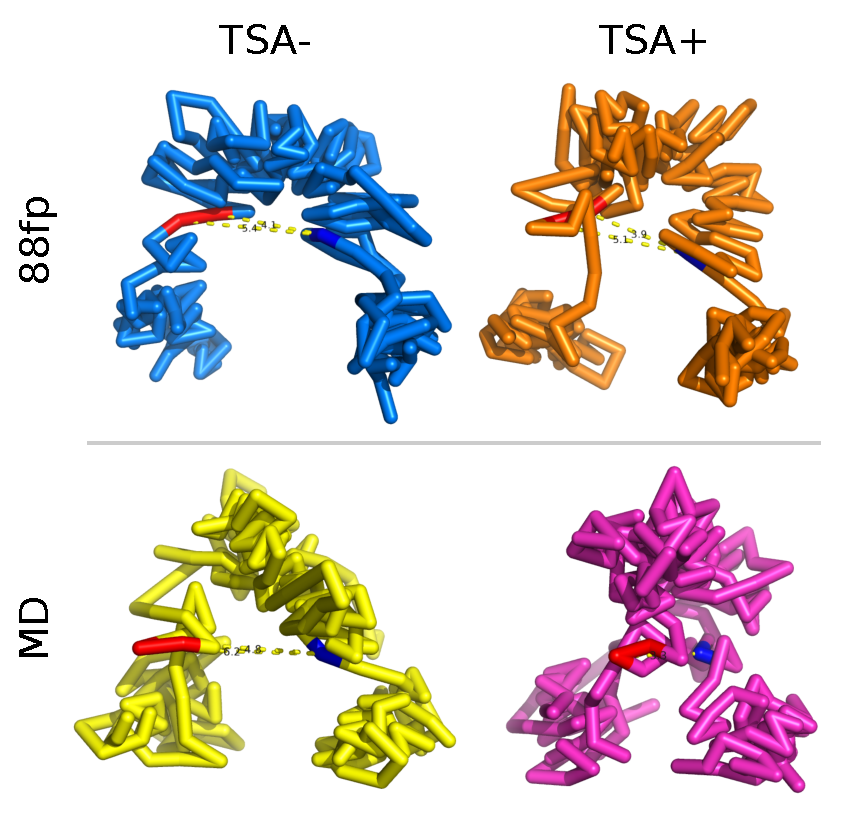
\includegraphics[width=5.45in]{5c3d.pdf}
\captionsetup{width=\textwidth} 
\caption[ Inferred polymer trajectories of the ZRS--\emph{Shh} region following TSA treatment in two cell lines. ]{ {\bf Inferred polymer trajectories of the ZRS--\emph{Shh} region following TSA treatment in two cell lines. }
3D structures are shown for 5C experiments assaying the region around \emph{Shh} (\emph{red}) and ZRS (\emph{blue}) in an \emph{Shh}-expressing limb bud cell line (88fp) and a non-expressing mandibular cell line (MD). Labelled measurements are given in Table \ref{tab:3ddist}. Structures were predicted by \texttt{AutoChrom3D}\cite{Peng2013} using $210 \times 8$ kb beads per polymer.
}\label{fig:5c3d}
\end{center} 
\end{figure} 

We find that TSA treatment of 88fp cells does appear to slightly reduce the distance between \emph{Shh} and ZRS in inferred 3D structures (Fig. \ref{fig:5c3d}), however this difference is overshadowed---to our surprise---by that observed in the non-expressing MD cell line. This latter mandibular cell line undergoes a large structural transition which brings the \emph{Shh} gene and ZRS into close proximity. Measurements between these elements for each structure are shown in Table \ref{tab:3ddist}.

We also report a greater overall structural shift following TSA treatment in the MD cell line, with an RMSD between the two structures of $2.377$ arbitrary units, relative to $1.701$ between TSA+ and TSA- 88fp cells. The radius of gyration, unchanged in 88fp, is also decreased in the MD cell line following TSA treatment, indicating the region becomes more compact following TSA treatment (Table \ref{tab:3ddist}).

\begin{table}[]
\centering
\caption[Measurement distances between ZRS and \emph{Shh} in each inferred 3D structure.]{ {\bf Measurement distances between ZRS and \emph{Shh} in each inferred 3D structure. }
Distances are given in arbitrary units. \emph{Shh} spans two beads of the polymer model, hence two distances are calculated in each case ($d_1$, $d_2$). RMSD is the minimised root mean squared deviation between the two structures and is given as a relative unitless quantity. The radius of gyration (gyradius) is also shown.
}
\label{tab:3ddist}
\begin{tabular}{ll|cc|l|cc|}
                      &    & \multicolumn{2}{c|}{{\bf Distance}} & \multirow{2}{*}{RMSD}   & \multicolumn{2}{c|}{{\bf Gyradius } ($\mu$m)}             \\
                      &    & TSA-             & TSA+             &                        & TSA-                   & TSA+                   \\ \hline
\multirow{2}{*}{88fp} & $d_1$ & 5.4              & 5.1              & \multirow{2}{*}{1.701} & \multirow{2}{*}{0.244} & \multirow{2}{*}{0.244} \\
                      & $d_2$ & 4.1              & 3.9              &                        &                        &                        \\ \hline
\multirow{2}{*}{MD}   & $d_1$ & 6.2              & 3.3              & \multirow{2}{*}{2.377} & \multirow{2}{*}{0.217} & \multirow{2}{*}{0.205} \\
                      & $d_2$ & 4.8              & 2.0              &                        &                        &                        \\ \hline
\end{tabular}
\end{table}

\subsection{Repeat simulations}

We have shown what appears to be a structural shift in the ZRS--\emph{Shh} locus by 3D modelling predictions (Section \ref{sec:shh5c}). It is of interest to assess the stability and reproducibility of these results through repeat simulations of the polymer trajectory. At this point it is unclear whether the ZRS--\emph{Shh} bound state represents a firm consensus over the cell population, or an alternative structure with similar optimisation energy to that of the non-contacting state. 

%Due to the use of cell populations we cannot resolve whether such a contact is either constitutive in a certain proportion of cells under study, or an ephemeral yet commonly-occurring interaction.

We re-ran simulations of the 3D chromatin fibre in the ZRS--\emph{Shh} region a total of five times (Fig. \ref{fig:3dreps}). In each case, the algorithm generates the known ZRS--\emph{Shh} TAD as a compacted domain bookended by the two loci under study. This sanity check shows that the results are broadly compatible with our \emph{a priori} expectation of the region's structure given the 2D heatmap representation of 5C data (Fig. \ref{fig:shhtad}).

Repeat simulations indeed appear to recreate the induced ZRS--\emph{Shh} contact in the mandibular cell line (MD) following TSA treatment (Fig. \ref{fig:3dreps}). This is again surprising, as the MD cell lines do not express \emph{Shh} and so were included as a negative control, with no expected changes in local chromatin structure following TSA treatment. In repeat simulations of the 88fp cell line, a close analogue of the 14fp cell line used in 4C, we see relatively little change in distance between \emph{Shh} and ZRS (Fig. \ref{fig:3dreps}). 

\begin{figure}
\begin{center} 
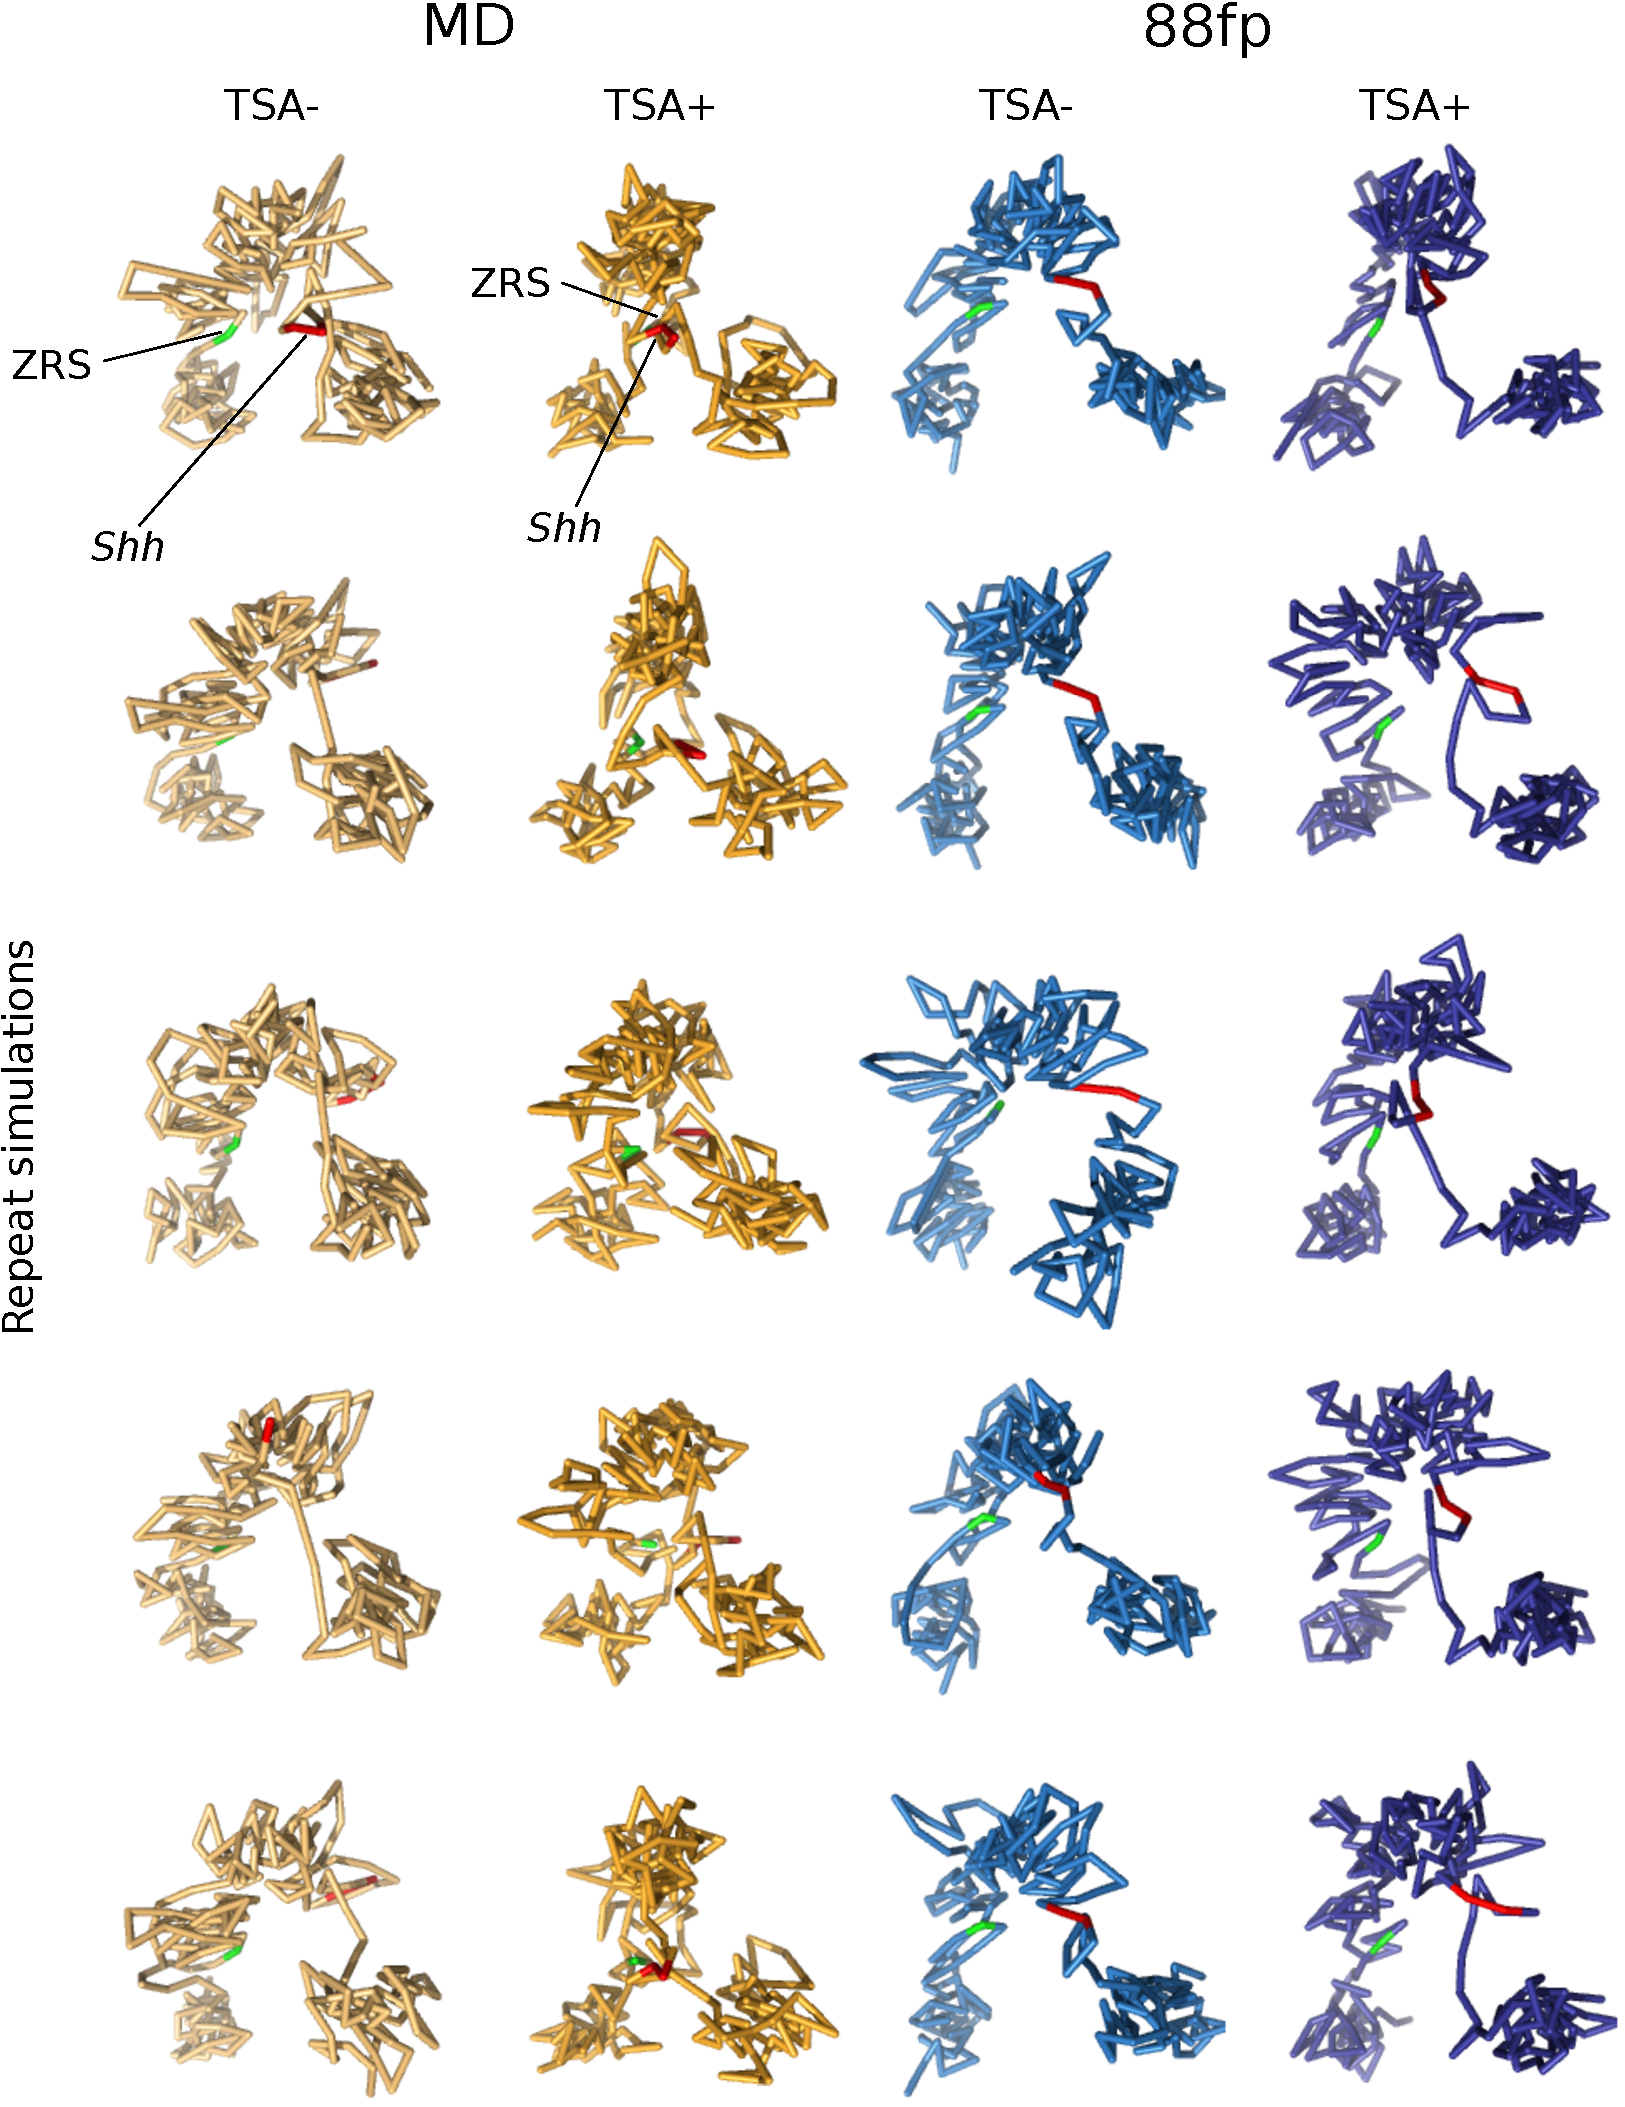
\includegraphics[width=5.45in]{3dreps.pdf}
\captionsetup{width=\textwidth} 
\caption[ Repeat simulations of 3D polymer trajectories in the ZRS--\emph{Shh} region. ]{ {\bf Repeat simulations of 3D polymer trajectories in the ZRS--\emph{Shh} region. }
3D structures are shown for 5C experiments assaying the region around \emph{Shh} (\emph{red}) and ZRS (\emph{green}) in an \emph{Shh}-expressing limb bud cell line (88fp) and a non-expressing mandibular cell line (MD). Structures were aligned as whole molecules to the uppermost replicate in each column.
}\label{fig:3dreps}
\end{center} 
\end{figure} 

We quantified these distances by measuring from the single bead containing ZRS to the two beads which overlap the \emph{Shh} gene (Fig. \ref{fig:3ddist}). While these are not biological replicates, just repeat simulations, we find the distance shift in MD cells is statistically significant at the level of $\alpha = 0.05$ for both bead distances (Mann-Whitney: $d_1: p < 0.012$, $d_2: p < 0.012 $). Distances in the 88fp cell line were not significantly different following TSA treatment (Fig. \ref{fig:3ddist}).

\begin{figure}
\begin{center} 
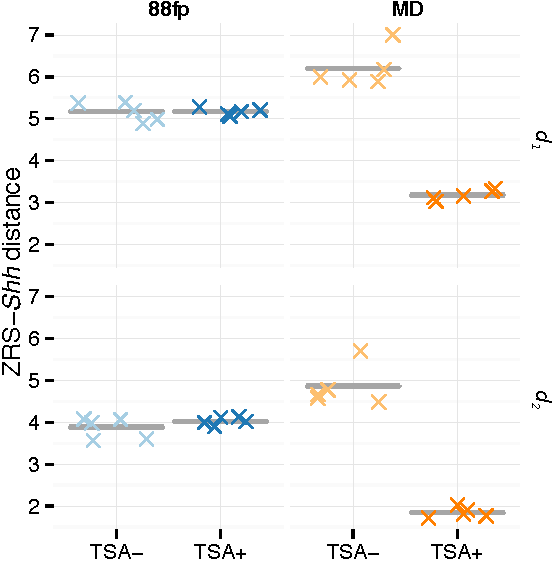
\includegraphics[width=2.75in]{3d_dists.pdf}
\captionsetup{width=\textwidth} 
\caption[ ZRS--\emph{Shh} distance measurements from repeated 3D polymer simulations. ]{ {\bf ZRS--\emph{Shh} distance measurements from repeated 3D polymer simulations. }
Measurements were taken from 5 replicate 3D simulations (shown in Figure \ref{fig:3dreps}). Distances are given in arbitrary units. \emph{Shh} spans two beads of the polymer model, hence two distances are calculated in each case ($d_1$, $d_2$).
}\label{fig:3ddist}
\end{center} 
\end{figure} 

Qualitatively, there could be some observable structural dynamics caused by TSA treatment in 88fp cells. It appears potentially that part of the \emph{Shh}--ZRS TAD becomes more loosely-packed at the ZRS side. This can be seen most clearly in two of the five simulations of the TSA treated 88fp polymer models (Fig. \ref{fig:decompaction}). Given the function of TSA as a histone deacetylase inhibitor, and unpublished results showing it causes an increase in H3K27 acetylation over the ZRS, we speculate that additional acetyl groups around this locus could be causing greater repulsion between histones leading to a less-compacted structure. Potentially then, the ZRS is transitioning to a more accessible state despite no change in its physical distance relative to \emph{Shh}.

\begin{figure}
\begin{center} 
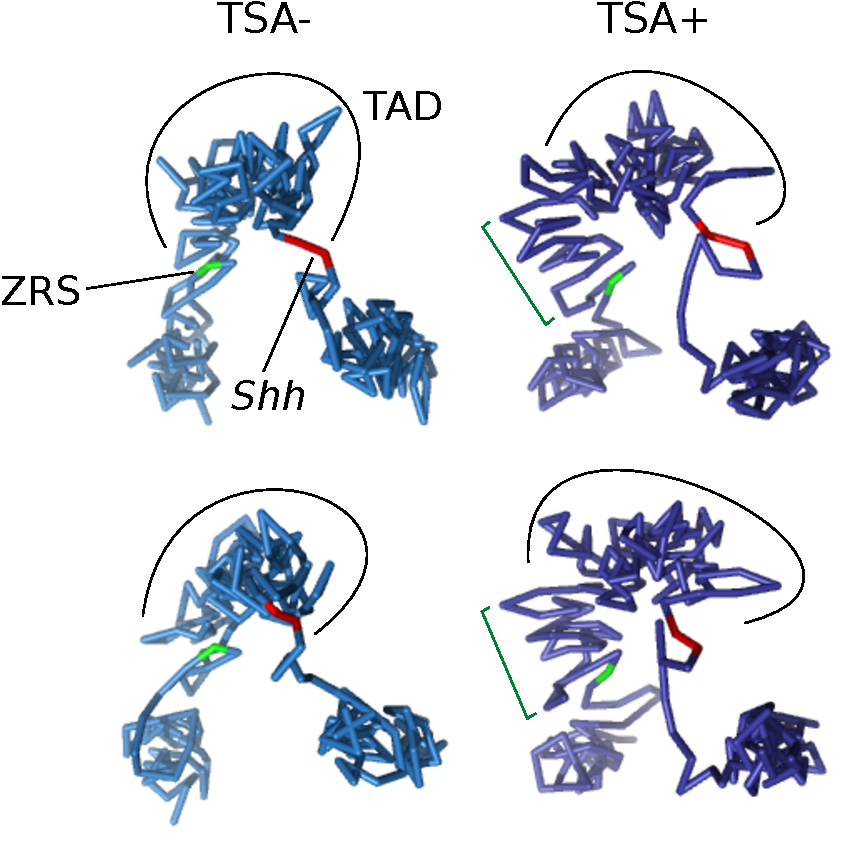
\includegraphics[width=3in]{decompaction.pdf}
\captionsetup{width=\textwidth} 
\caption[ Polymer models showing partial TAD decompaction following TSA treatment. ]{ {\bf Polymer models showing partial TAD decompaction following TSA treatment. }
Two of the simulations from Figure \ref{fig:3dreps} are shown here with additional annotation. In the TSA treated 14fp samples (TSA+) there is potentially evidence for a looser packing of the chromatin around the ZRS (\emph{dark green}).
}\label{fig:decompaction}
\end{center} 
\end{figure} 

%\subsection{Discussion}

The main result, that TSA treatment induces a \emph{Shh}--ZRS contact in mandibular cell lines but not in limb bud, is difficult to explain and runs contrary to our expectations. 4C experiments performed over the same region reported ZRS--\emph{Shh} contacts (Fig. \ref{fig:4carcs}) but polymer models using 5C found instead that these two loci remain relatively separated with or without TSA treatment (though still much closer than expected relative to their genomic distance; Fig. \ref{fig:5c3d}). One explanation for this could be the filtering method used by \texttt{AutoChrom3D} (Section \ref{sec:achrom}). Highly improbably contacts are filtered before structural prediction to prevent errors or artefacts leading to aberrant structures. In this case, a genuine instance of long-range \emph{cis}-regulation may end up being down-weighted or removed before polymer modelling. Alternatively this may be an example of where, as has been noted at high-resolution, the results of 5C as formaldehyde cross-linking efficiencies cannot be interpreted as spatial distances.\cite{Williamson2014}

%Firstly the \emph{Shh}--ZRS contact has previously been shown by 3D-FISH to be associated with \emph{Shh} expression in the developing limb bud, though it is not detected in every cell.\cite{Amano2009, Hill2013a} Instead only a proportion of cells in the ZPA are \emph{Shh}-expressing at a given time, and it is within these expressing cells where \emph{Shh}--ZRS colocalisation is most likely.\cite{Amano2009}


Additional follow-up experiments are underway to further explore the dynamics in this region.




\ifstandalone
\begin{small}
\bibliography{/Users/benmoore/Documents/library,/Users/benmoore/Documents/customrefs}
\end{small}
\fi

\end{document}
